\chapter{Development and\\Implementation}
\label{cha:implementation}
\chapterquote{It's done, when it's done}{An English Phrase}

\section{Outline}
The sections in this chapter will describe the various stages of development and implementation of this Bachelor thesis' application. At first the basic idea of the layout and the individual views will be described and explained. To get an even better impression the early paper prototype will be shown. Afterwards a short description of the aspired time schedule for the development as well as the creation of the written elaboration is given.

The implementation of the basic layout which was displayed and explained with the help of the paper prototype, will be the first part describing the actual implementation process.
Second, the handling of the data to be visualized is explained. This covers the server based access as well as local storing and loading. 

After the preparations for the visualization have been set forth, the different views will be described. Starting with the explanation of the map view, it will be clarified how the loaded data is visualized. This is followed by the section focusing on the chart view. It explains how a library is used to draw pie charts and how the loaded data has to be prepared. The last section describes how the timeline was implemented. It covers, how one can draw its own views in Android and how to make use of gestures.
\newpage
\section{Paper Prototype}
\label{sec:paper_prototype}
The first step of the development process was the creation of a paper prototype. It was needed to demonstrate the idea and visual appearance of the project and application. Another advantage of the paper prototype is to be able to show the application to  different people and to get feedback without even writing one line of code. This provides the ability to eliminate possible false estimations  in the forefront of the application's implementation. False estimations may be the assumption of wrong needs of possible future users or the creation of an non intuitive layout. In the following the paper prototype will be shown and explained.

The\mnote{Basic layout} first idea was to split the screen into two parts, an option part and a view part. The left part should be the option part, occupying one sixth of the visible screen. It should always display the following, in appearing order listed, options.\\
In the top left a view selection containing three buttons  ordered vertically with titles ``Map-View'', ``Chart-View'' and ``Timeline'' are displayed. Taping one of those buttons causes a view switch to display the respective view.\\
Under the view selection a list of options should be visible. Those options vary from view to view but should always contain a button at the top of the list displaying the currently selected date. Tapping on this button causes a date-selection-window to pop up. Selecting a date leads to an update of the displayed view, now visualizing the respective data.
Other options will be explained together with their respective views.

When \mnote{Map-View} the application has been loaded, the user will be displayed the map view thus making it the application's start view. The view will display a map with a route, representing the user's visited locations. On start up the selected date will be the current day and therefor the draw route represents the user's latest movements. Tapping on the route should bring up a speech bubble which contains information about the tapped location. Those informations will be the time spend on that location, the used applications and possibly shot photos.\\
The \mnote{Map-View specific options} view provides two special options. The first option is represented by a check box and has the title ``Photos''. The option provides the ability to highlight those locations, where a photo was taken. The second option is called ``Apps''. It lets the user pick applications from a list and colors all parts of the route where those specified applications were used. Those options would provide a great tool to quickly get an overview over the position data of specific applications and actions. An actual image of the paper prototype for the map view can be found in figure \ref{img:mapview}.

The map view can mainly be used to answer the question ``Where was smartphone used?'', since the view focuses on visualize the map and traveled routes rather than displaying numbers and percentages.
\begin{figure}[h]
	\caption{Map-View}
	\label{img:mapview}
	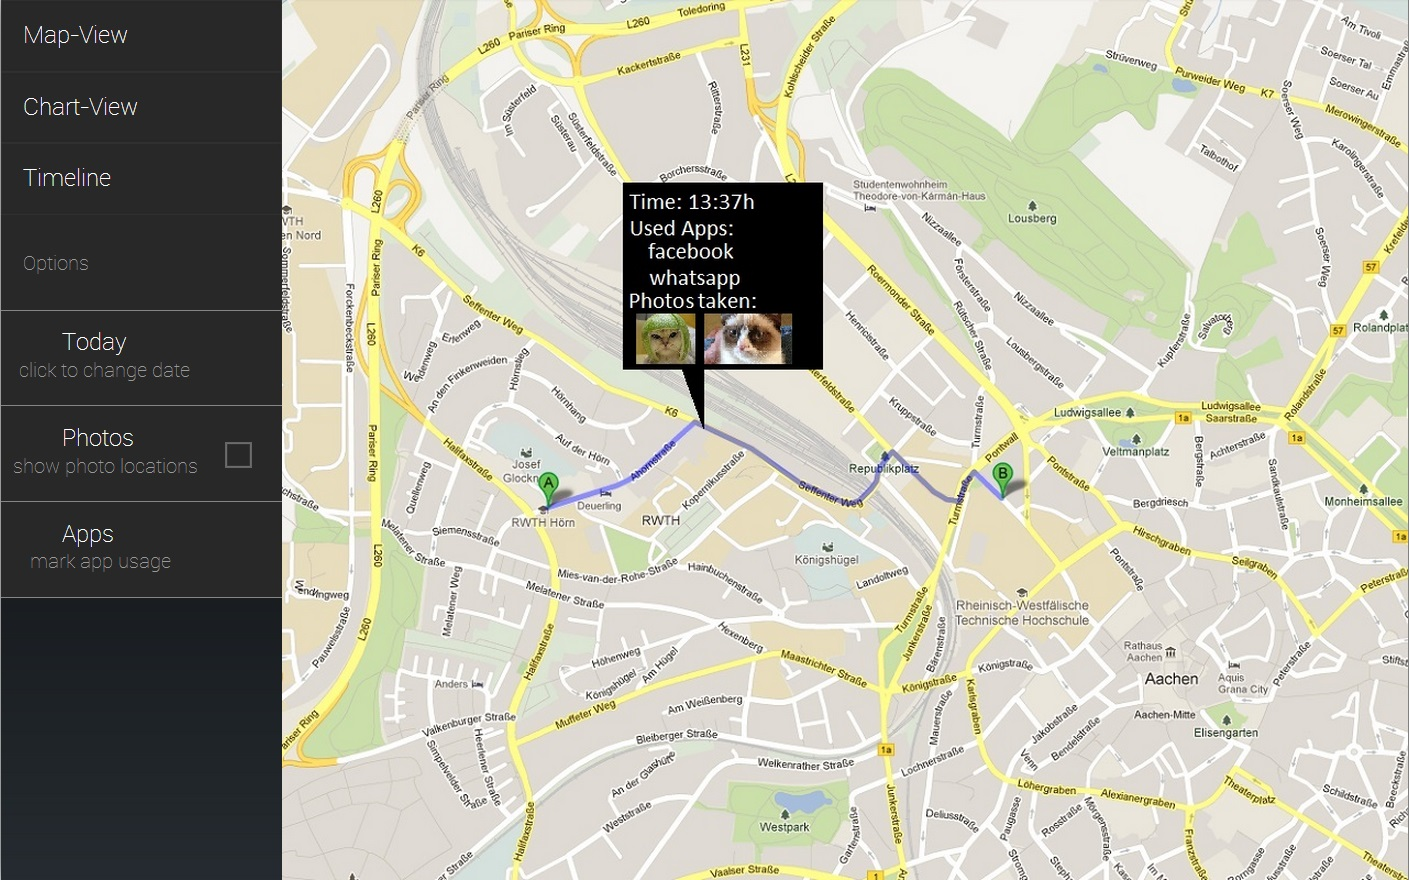
\includegraphics[width=\textwidth]{images/Design/1b_onClickPageView.jpg}
\end{figure}

The \mnote{Chart-View} second view, the chart view, shows the user his or hers daily activities in form of a pie chart. Its layout can be found in figure \ref{img:chartview}. The idea was to create location based charts that shows for each visited place the percentages of used applications. To break down the number of shown charts and thus to give a better overview, locations would be summarized in an intuitive way. That means that one has a chart for work, home and on the move. Those charts are lined up vertically and have an individual chart on the top of the list. This individual chart can be adjusted by the two extra options described in the following.\\
The \mnote{Chart-View specific options} first option lets one choose which places are taken into account for the individual chart. The second option determines which specific applications are displayed in the first chart. With these two options, one has the ability to to customize the first chart to visualize only those data which fit one's individual needs.

To \mnote{Grouping of apps and locations} get an even better overview, applications are classified into different groups. ``Social'' and ``Productive'' could be two groups, which split the applications apart. Applications like whatsapp and facebook may be social, while mail programs would be productive. The user would also be able to classify the applications by him- or herself, allowing to personalize the application. Furthermore, home, work and other places are chosen individually and extra places like parent's home can be added by the user, to give the him or her more space for customization.

To \mnote{Interacting with the view} get an better insight of the application groups, tapping on a slice of the pie chart will bring up a detailed view. In this detail view, one can see which applications are included in the tapped group and how large their percentage of daily activities is. In addition the total usage time of each application is shown, to give the displayed percentages more expressiveness.

The chart view, in contrast to the map view, is able to give a better overview over the percentages of used applications rather than show in which locations they have been utilized. It gives answer to the question ``What was the smartphone used for?''
\begin{figure}[h]
	\caption{Chart-View}
	\label{img:chartview}
	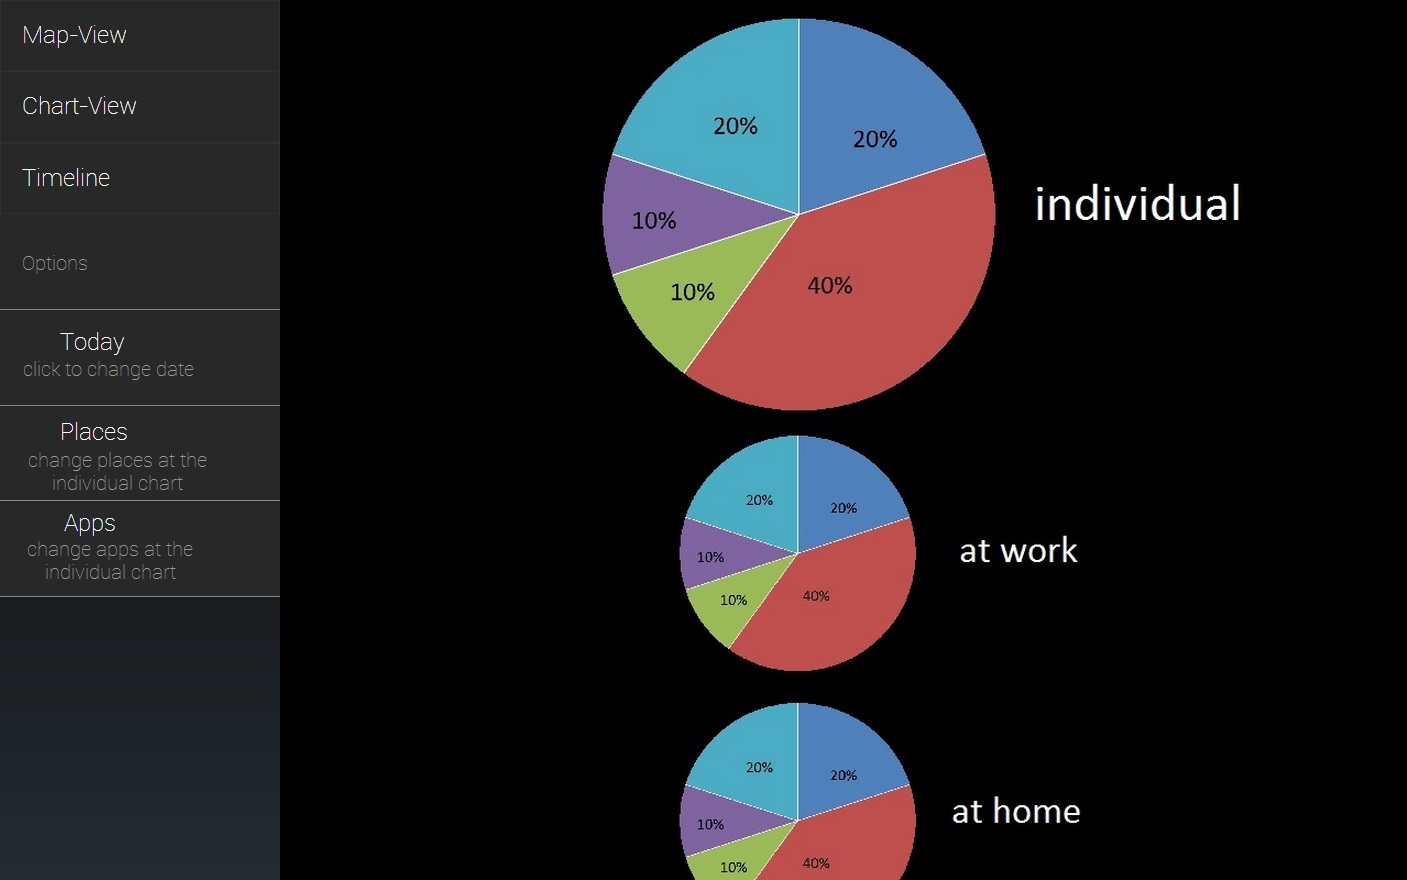
\includegraphics[width=\textwidth]{images/Design/2_ChartView.jpg}
\end{figure}

The \mnote{Timeline} timeline is the third and last view of this thesis' application. For a visual representation of the description of this view, please refer to figure \ref{img:timeline}. This view visualizes the daily activities in a chronological manner with two major parts. The first part is the the timeline itself and is described as follows. At the layout's bottom a horizontal line is draw with markings for every hour, from 0:00 to 24:00. Above this line, colored rectangles are drawn which represent a timespan in which an application was used. At the layout's top one can see markings for the visited location in dependence of the displayed timespan. One has the possibility to scroll horizontally through the view to observe the consecutively occur activities.

Beneath \mnote{The detailed view} the actual timeline a detailed view of all applications used on the selected date is found. This second part shows the application in descending order starting with the application mostly used on the chosen date. For each application a rectangle which represents the percentage of daily usage, is drawn. This rectangle will have the same color as the respective rectangles in the timeline and thus the detailed view can be used as a legend to identify the applications displayed in the timeline. Next to the application's bar the respective percentage and total amount of time is displayed.

This \mnote{Timeline specific options} view offers the extra option ``Apps'', where one can filter the displayed applications. With that option one is able to hide all other applications and display only those which are relevant for the user and thus giving the application a feel of personality and individuality.

Although it partially acts as a bar chart, the timeline, unlike the other views, focuses on the daily schedule by visualize the activities in a chronological order. With this view the user is able to answers the question ``When was the smartphone used?''.
\begin{figure}[h]
	\caption{Timeline}
	\label{img:timeline}
	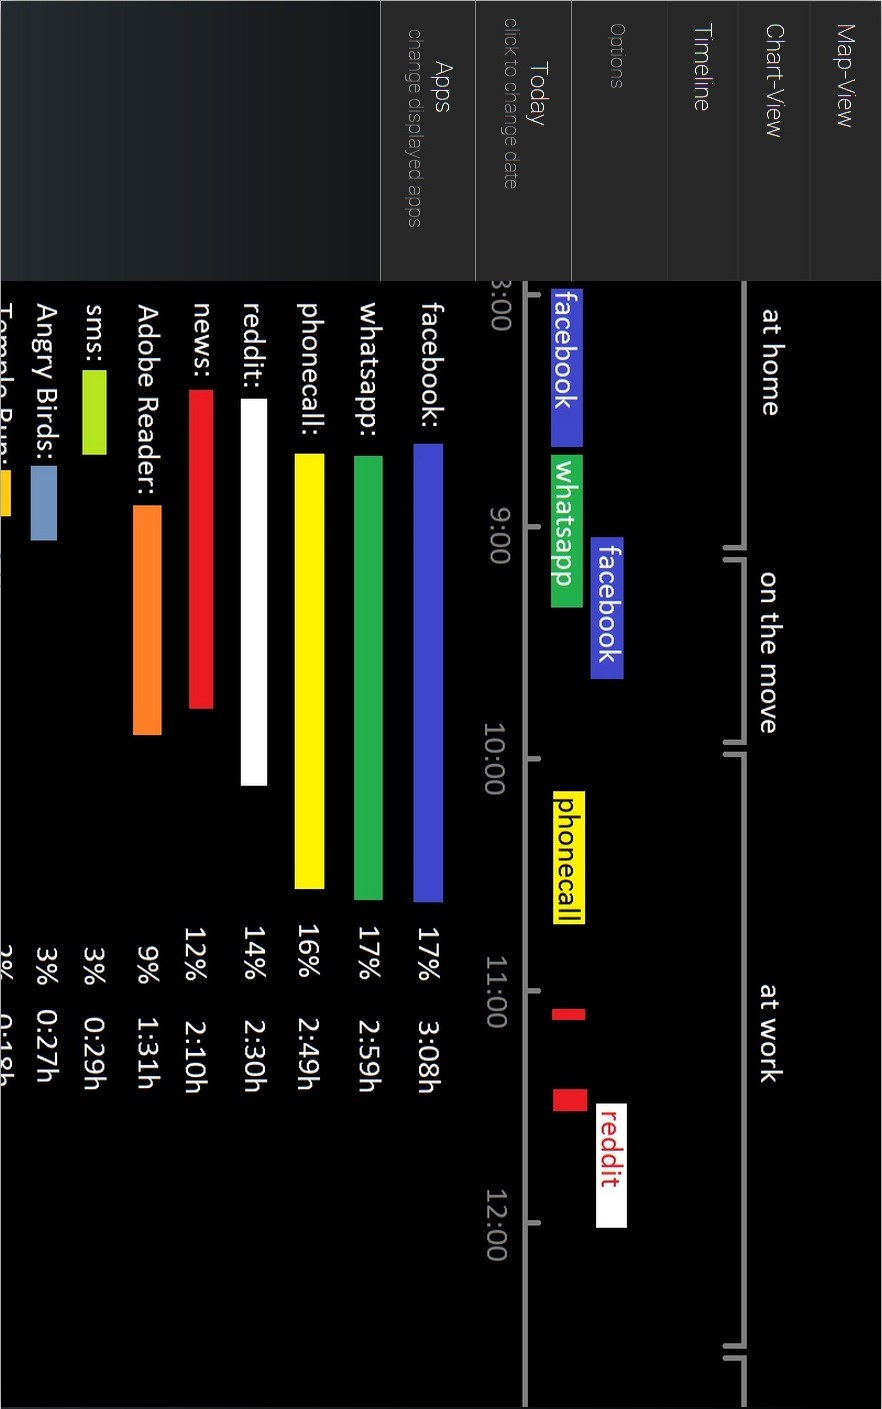
\includegraphics[width=\textwidth]{images/Design/3_TimeLine.jpg}
\end{figure}

As mentioned in the first place, this was the basic idea of the application and a few things have been changed during the development process. A summary of changes which differ from the paper prototype, along with the reasons for those changes can be found in the next sections.

%\newpage
%\section{Time Schedule}
%\label{subsec:time_schedule}
%For the proposal of this bachelor thesis a time schedule was created to structure the work flow. The estimated durations for each major task can be found in figure \ref{ganttchart1}.
%\begin{figure}[h]
%\begin{minipage}[][][c]{\textwidth}
%\caption{Gantt Chart: time schedule}
%\label{ganttchart1}
%\begin{ganttchart}{1}{17}
%	\gantttitle{Weeks}{17} \\
%	\gantttitlelist{1,...,17}{1} \\
%	\ganttbar{Research}{1}{2} \\
%	\ganttbar{Design Concept}{2}{4} \\
%	\ganttbar{Basic GUI}{3}{3} \\
%	\ganttbar{Chart View}{4}{5} \\
%	\ganttbar{Data Management}{6}{8}\\
%	\ganttbar{Timeline}{8}{9}\\
%	\ganttbar{Map View}{10}{11}\\
%	\ganttbar{Written Elaboration}{11}{17}
%\end{ganttchart}
%\end{minipage}
%\end{figure}
%
%The shown estimations were not always correct. The first weeks of this project went as planned and the incorporation in Android ran without greater problems. Likewise was the task of designing the paper prototype. In fact, the paper prototype took only one and a half weeks, therefore one had more time to focus on the basic user interface and the chart view.
%With start of the fifth week, the chart view was set up and first steps for data management were made. Unfortunately implementing the accessing of data, downloading, processing and storing took longer than expected, but the previously gained extra week could compensate it.\\
%The implementation of the timeline and the map view went as planned, but the writing of the written elaboration was not started until the 13. week due to polishing of visible and non visible parts of the application. Details about the progress of specific implementation parts are described in the next sections. 
\newpage
\section{Basic Layout}
	\label{sec:basiclayout}
The actual implementation work started with the creation of the basic layout. It characterizes the general picture of the application and has changed during the process of implementation.

%talk about lifecycle, provided views and viewgroups
When \mnote{View, Viewgroups and Fragments} the application first starts, one has to pass a layout to the main process, the main activity, to create a visible view. Those layouts are defined in xml and contain views and viewgroups. Basically, viewgroups contain views and/or other viewgroups and define their layout. For example one can define, whether visible views are ordered horizontally or vertically. Views contain the actual visible content, for instance a text or an image. Views are not static objects and can change during run time. One is also able to create and delete views and viewgroups during runtime, which will be helpful later. In order to create an application which looks and works like the paper prototype, one has to be able to change or switch whole groups of views in order to switch between map view, chart view and timeline. For this purpose one can use fragments.Fragments are kind of sub-activities which handle their own lifecycle and viewgroups and they are necessary for an interactive application, as they can be reused during runtime, thus provide an efficient way for switching views.

The first basic layout can be found in figure \ref{img:firstbasiclayout}. It resembles the paper prototype in functionality and appearance. Tapping on the view's name causes a view switch and options bring up pop up menus to select applications or a date.
To provide the application with the ability to react to user input, one can assign click listeners to views. After creating and assigning a click listener, Android calls it as soon as the user taps on an assigned view and a specified action, for instance a view switch, will be performed.
\begin{figure}[h]
	\caption{First Basic Layout}
	\label{img:firstbasiclayout}
	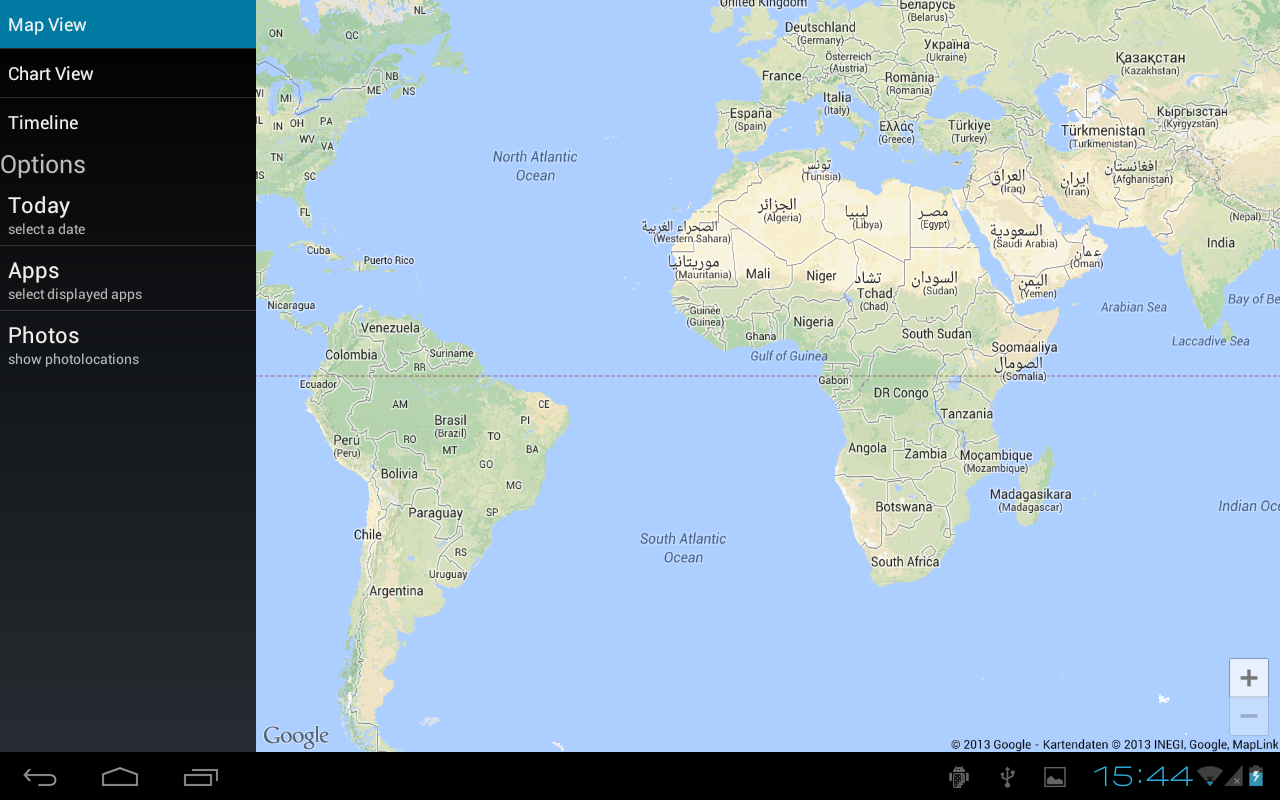
\includegraphics[width=\textwidth]{images/Screenshots/v3/Screenshot_2013-08-19-15-44-21.png}
\end{figure}

As \mnote{Visible fragments} mentioned above, at the start of the application the main activity needs a layout in order to create visible content. In this case the layout consists of three fragments. The first fragment is the view selection fragment. This is a list fragment which contains the three section names as views. The list fragment provides the programmer with the function \lstinline[language=Java]$onListItemClick$ which he or she can override. It gets called if one of the views names get clicked and is provided, among others, with the list position of the clicked view. With this information one is able to determine which view is requested and can then call the main activity to initiate a switch.\\
The second second fragment is the options fragment which is also a list fragment with the same abilities as the view selection fragment. If the user taps on an option the respective menu pops up and if the user makes adjustments the underlying dataset is updated and the main activity gets called to update the currently visible views.\\
The last fragment and most important in case of visualization and self reflection is the view section fragment. Those fragments visualize own layouts with different views which are described in their respective section.

In \mnote{Add and switch fragments} the first layout, the view selection fragment called the main activity in order to switch the view section fragment. To switch fragments the main activity uses the FragmentManager api. To obtain a FragmentManager object, the main activity calls \lstinline[language=Java]$getFragmentManager()$. With this object one can access a FragmentTransaction object, which is used to add or replace fragments. With the FragmentTransaction's function \lstinline$add(int, Fragment, String)$ one adds a fragment to a specific view. Do do so, one has to specify the container in which the fragment will be placed via an integer id previously assigned, the fragment to add to the container and an optional tag to access the fragment later. With a call of FragmentTransaction's function \lstinline$commit()$ the transaction will be executed.\\
To switch a fragment, one calls the FragmentTransaction's function \lstinline$replace(int, Fragment, String)$ with the same variables as previously described. It should be mentioned that only those fragments can be replaced that were added in a programmatically way and were not defined in the xml's layout file. Instead if just adding a new fragment to an occupied container one should use the \lstinline$replace()$ function or otherwise it can not be guaranteed that only one fragment is visible. But because \lstinline$replace()$ destroys the fragment, its rather inefficient if a user switches views very often, due to the fact that the fragment will be recreated every time it is added.\\
A solution to this problem are the FragmentTransaction's \lstinline$show()$ and \lstinline$hide()$ functions. These functions obviously show and hide fragments without destroying them, therefore they are more efficient in case of power consumption and calculation time. Another advantage is the maintaining of zoom and scroll positions without adding a single line of code.

To \mnote{Dialogs and DialogFragments} change the fragment's appearance, one can tap on the options on the left side to bring up a pop up menu with a calendar or a checklist of application names. These option menus are created with Android's Dialog objects and controlled by the DialogFragment api. The first options menu, the calendar, is displayed by a special dialog, the DatePickerDialog which provides a visual appealing user interface to select a date. Once the option fragment created a DialogFragment, it has to assign itself as a listener to the object and call \lstinline$show()$ to Display the graphical user interface. To be able to handle the choice of a date, the DialogFragment implements DatePickerDialog's \lstinline$OnDateSetListener$, which gets called with the selected year, month and day if the user approves his or hers chosen date. Afterwards the DialogFragment calls the previous assigned listener and passes the the date to it. The options fragment then displays the selected date and stores it in the dataset, which notifies the main activity to update all visible fragments.\\
The other pop up options menu is also Dialog managed by a DialogFragment. It displays application names with a check box. To show this dialog, the options fragment creates a DialogFragment object and calls \lstinline$show()$. The options fragment does not have to assign itself as a listener but has to select a mode for the DialogFragment in order to load, display and store data correctly. Those modes are select\_apps, ignore\_apps and select\_highlight\_apps. Each mode builds its dialog identically with the help of a dialog builder. This builder offers different functions to create various dialogs and in this case is used to create a dialog with a multiple choice list and two buttons on the bottom. The builder provides a function called \lstinline$setMultiChoiceItems()$ with the following input variables. A string array of application names, an array of booleans representing checked states of the applications and a listener to handle click events. The application names and the boolean arrays are different for every mode, as they are loaded and gathered differently, for example the select\_apps mode only displays names of applications used at the currently selected date and forgets the selections after a restart, whereas the ignore\_apps mode loads all application names ever used by the owner an stores the selections in the dataset. The assigned listener tracks selection and deselection of list items and stores the application's name and the respective boolean for every change. If the user confirms his or hers selection, the dialog then stores according to the chosen mode, the selections in the dataset which again tells the main activity to update the fragments.

As \mnote{Change of the basic layout's visual appearance} the process of development progressed, the need of more options than previously assumed raised. Options for colorization of applications, switching the logged in user, deleting local files and permanently ignoring applications needed to be assigned to the layout. The problem with these options were, that they would not be used as much as selecting a date or temporarily hide displayed applications. Adding the options under the existing ones would cause a loss in simplicity and clarity of the application. The solution was Android's ActionBar api.

The ActionBar serves as a navigation bar which is set up at the top of the application and lets the programmer add tabs and option buttons, where option buttons can also be combined in small pop up menu. 
\begin{figure}[h]
	\caption{Final Basic Layout}
	\label{img:finalbasiclayout}
	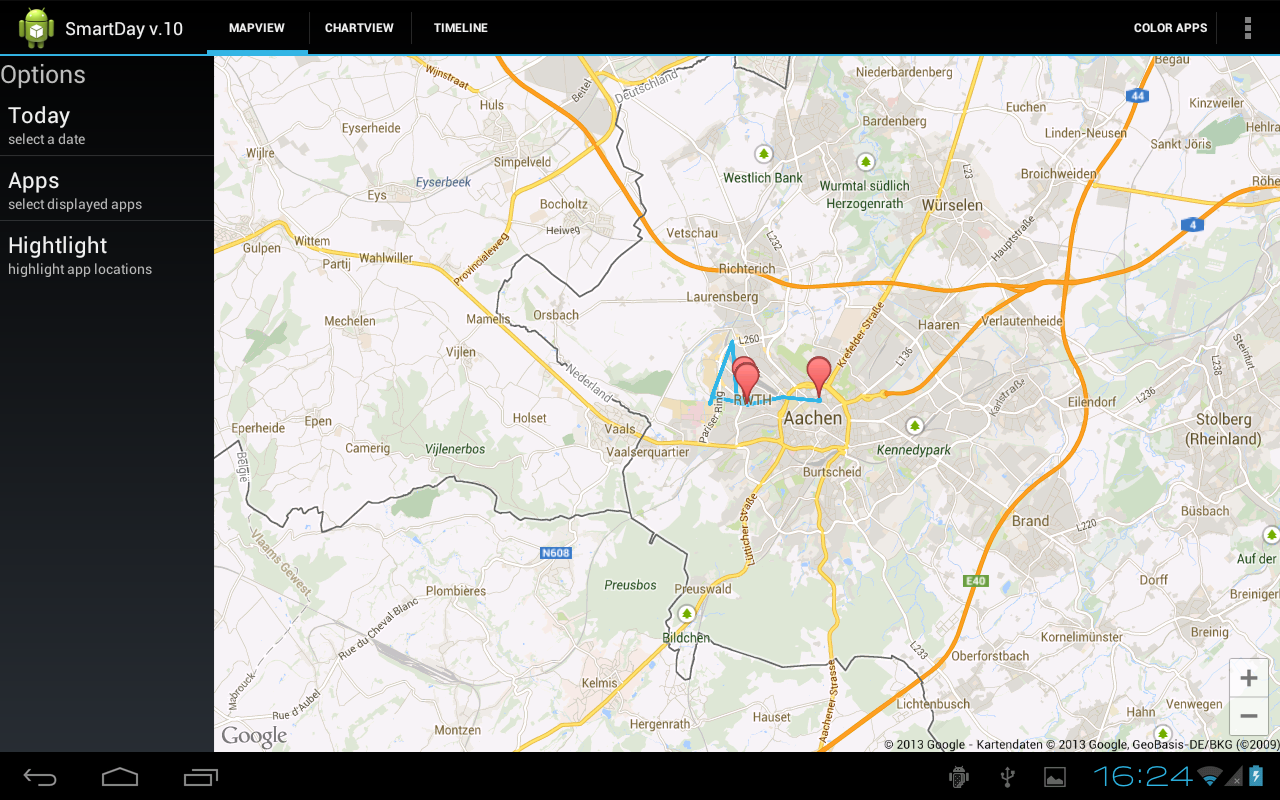
\includegraphics[width=\textwidth]{images/Screenshots/v10/Screenshot_2013-08-19-16-24-58.png}
\end{figure}

In \mnote{The action bar} order to make full use of the now used ActionBar, the former view selection fragment was deleted and the view's are now selected on the action bar by tapping on the new tab header. This layout is more intuitive as it resembles know patterns of Internet browsers and feels more structured. On the right side of the action bar, the color apps button is visible next to three dots which open a small list with the other new options - switch user, delete saved files and ignore apps. For more details see figure \ref{img:finalbasiclayout}.

The \mnote{Action bar tab header} main activity controls and sets up the bar as follows. By default, the action bar is visible in the application's layout but does not contain anything than the application's name in the top left corner. To add tab headers and options, one has to work with the ActionBar api. The main activity calls the function \lstinline$getActionBar()$, which returns an ActionBar object. With this object one can call the ActionBar's function \lstinline$newTab()$ to construct a new Tab object, which then has to be provided with a title via \lstinline$setText(String)$ and in order to react to taps, with a TabListener. In this thesis' application the TabListener class which implements the ActionBar's TabListener interface and manages its own tab and the respective fragment. The reference to the TabListeners are saved in the main activity, such that it can programmatically select or reselect a specific tab to notify changes or just to switch the tab. Once the data is provided, one can add the tabs to the ActionBar with a call of the ActionBar's function \lstinline$addTab(Tab)$.

Option buttons \mnote{Action bar option buttons} for the action bar are declared in an xml file. In this application the xml nodes representing the buttons by four key value pairs.
The first entry is an id, which is used to refer to the button from within the programs code. The title of the button is given in the field of the same name. A priority number to define the order of appearance of the buttons and an option to define if the button should be grouped under the three dots list or if it should directly be accessible on the action bar.\\
The main activity then has to override the function \lstinline$onOptionsItemSelcted()$ which gets the tapped button as input. With the previously assigned ids, one can differentiate between the four buttons and execute their respective functions which will be explained in the following.

The \mnote{Switch user} ``Switch User'' button allows the user to switch the profile accessing the visualized data. If this button is tapped, the main activity looks up if the user had stored his or her login information and deletes them. Then the underlying dataset function \lstinline$createNewUser()$ is called and the user is asked to provide new login data. The mentioned data set and its corresponding functions will be explained in section \ref{sec:datamanagement}.\\
``Delete Files'' \mnote{Delete files} gives the user the ability to regain occupied memory storage by deleting saved files. The main activity looks up the applications file directory and deletes any stored file, excluding the user login data. Those stored files are downloaded information about days along with colorings of displayed applications and the selection of ignored applications.\\
In \mnote{Ignore applications} order to permanently remove applications from selections and views, one can tap the ``Ignore Apps'' button. This causes the main application to request every used application from the dataset by calling \lstinline$getAllApps()$. After the dataset has downloaded all application names from the server, the main activity creates a dialog where the user can pick applications which will be hidden permanently. The selection will then be stored in the dataset and all views will be updated.\\
The \mnote{Color apps} button which is visible as long as the screen sizes offers enough space, is the ``Color Apps'' button. Tapping this button causes the main activity to create a dialog displaying application names with respectively colored rectangles next to them. A tap on the application name or rectangle unveils a new pop up menu which lets the user pick a color as seen in figure \ref{img:colorpicker}.
\begin{figure}[h]
	\caption{Color picker}
	\label{img:colorpicker}
	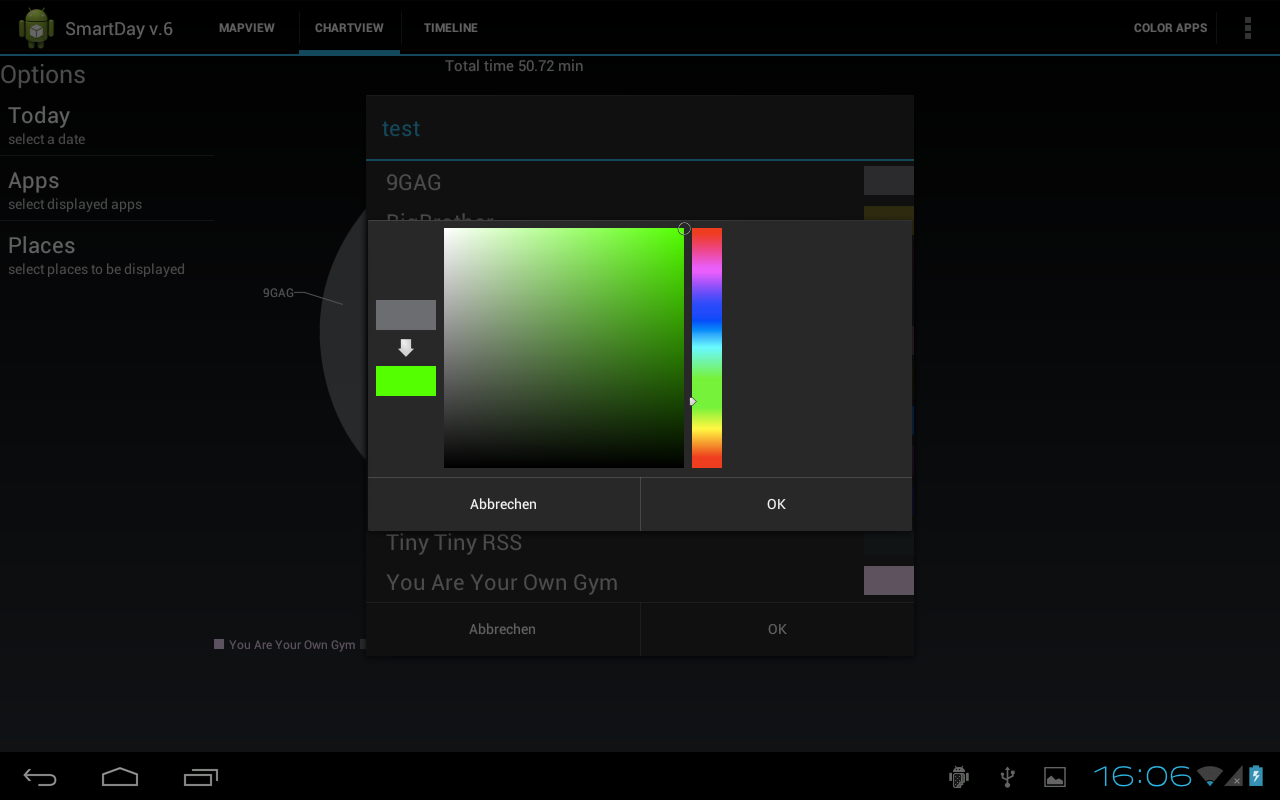
\includegraphics[width=\textwidth]{images/Screenshots/v6/Screenshot_2013-08-19-16-06-13.png}
\end{figure}

This new pop up is built with Yuku Sugianto's Android Color Picker or the Indonesian translation Ambil Warna\cite{colorpicker}. To use this color picker, one has to include the source code into its own application code and define it as a library project in order to access functions and classes. Once the Ambil Warna was linked as a library project, the application uses it as follows. As soon as an application name or the respective rectangle is tapped, the \lstinline$onClickListener$ extracts its own title, which is the applications name and creates an \lstinline$OnAmbilWarnaListener$ which overwrites the functions \lstinline$onOk()$ and \lstinline$onCancel()$ which are listeners and get called if their respective button is tapped. If \lstinline$onOk()$ is called, the function stores the color and respective application name and afterwards updates the color of the rectangle.\\
After \mnote{The AmbilWarnaDialog} the construction of the \lstinline$OnAmbilWarnaListener$, the \lstinline$AmbilWarnaDialog$ will be created by passing the current activity, the start color and the listener. With a call of \lstinline$show()$ the dialog is displayed and the user can interact with it. Once the user has picked all colors and hits ok, the dialog stores the new colors in the data set which then notifies the main activity to update its fragments. If the user decides that he or she does not want to apply the changes and taps cancel, all changes are discarded.

The basic layout is an essential part of the application experience. It offers not only a structured layout for view corresponding options and general ones, but it also presents a surrounding structure for views themselves. The possibility to seamlessly attach new views with tab headers and options on the left option fragment without destroying the uniform appearance of the application may be an advantage for possible future projects.\\
The basic layout was created to be minimal in terms of displayed options in order to prevent distraction from the actual function of this application, the self reflection.
\newpage
\section{Data Management}
\label{sec:datamanagement}
In the last section the term of a data set was mentioned a few times. This data set or the managing class of it will be explained in this section. It is the essential for the whole application, as it provides every fragment with the needed user data. The construction of this class was one of the hardest part of developing SmartDay and pieces of it were rewritten or removed as the development of the different fragments proceeded. Especially notifications for the main activity in order to update views if new data was available have been adjusted a few times.

The \mnote{JSON format} application's underlying dataset is stored in a \emph{JavScript Object Notation}, in short JSON, format. JSON structures consist of  key:value pairs, where the value can be a number, string, object or array. Keys and strings are enclosed by quotation marks and the key is separated from the value by a colon. An object is enclosed by curly braces and contains a collection of key:value pairs, each separated with a comma. An array is a collection of objects, each separated by a comma and enclosed by square brackets. JSON offered an easy way to handle the data provided by the server and was also natively supported by Android. The following sample describes the actual structure of the JSON object which is primarily used by the application and can be seen in figure \ref{fig:jsonobject}.
\begin{figure}
\caption{The Basic JSON Object}
\label{fig:jsonobject}
\begin{lstlisting}[language=json,firstnumber=1]
{ "dateTimestamp": long,
  "downloadTimestamp": long,
  "totalDuration": long,
  "result":[
    { "app": string,
      "duration": long,
      "usage":[
          { "session": string,
            "start": long,
            "end": long,
            "location":[
                 {"key": "lat",
                  "value": long
                 },
                 {"key": "lng",
                  "value": long
                 }
            ]}, ...
      ]}, ...
  ]
}
\end{lstlisting}
\end{figure}

In \mnote{JSON object in SmartDay} the top level object, the structure holds informations about download and date time stamp, along with the total time of application usages. In this application, all information about time are given in seconds precision. The JSON object holds an array called result and contains a JSON object for every application used at the specific day. Each of these objects contains a field app with the application's name stored as a string and a field duration, containing the total duration time of the application. Each object also contains an array \emph{usage}. This array contains objects of every timespan in which the application was used. Every usage object contains keys start and end with respective time stamps for start and end time. In addition the field session contains the applications session id and an array \emph{location} is given which contains two objects. These objects contain a key:value pair key which identifies whether the object holds information about the longitude or latitude, by storing a string with content lng respectively lat. The actual position information is stored in the value field which stores it as double.\\
With these information one has all needed data to create the fragments reflecting one's daily activities.

The \mnote{DataSet initialization} data managing class \emph{DataSet} is designed to be a singleton to guarantee that every view and fragment of the application is provided with the same data. In order to obtain a \lstinline$DataSet$ instance, one can call \lstinline$getInstance()$ which returns an instance of \lstinline$DataSet$ or initializes one and returns it, if none exists. In the process of initialization, the instance requests a new object of the class \lstinline$UserData$ which holds the user name and password. While the \lstinline$UserData$ object is created, it is directly checked, if the data is correct by contacting the server, but this will be explained later in this section. After requesting user data, it is checked, whether data for colorization and for ignoring applications are stored locally and can be loaded or not. If files are available, they are read and respective JSON objects are created and stored. After \lstinline$UserData$ calls \lstinline$DataSet$ to pass a successfully created and tested user object it is stored and the date is initialized. Since the application provides support to display data of multiple days in one fragment, the current date is determined, stored and selected as start and end date, meaning that at the time of initialization only one date, the current day is selected. Storing of the current date is only necessary to check if a chosen date equals the current date and thus label it as ``Today''.\\
Once the initialization part and therefore the creation of the \lstinline$DataSet$ instance is completed, the instance calls its own function \lstinline$getApps(Listener)$ with \lstinline$null$ as listener. This function requests a download of data of the selected day and the reason for the call with \lstinline$null$ is, that in this way the main activity is notified that the data is available for first time and it can set up the fragments for the first time which need the data.

As mentioned, \mnote{Creating a new user} the a new user object is requested from \lstinline$UserData$. This is done by calling \lstinline$getUserLoginData$. This function is provided with the main activity and an optional boolean as parameters. The main activity is needed to for different functionalities like storing data in a local file or accessing the Internet, which is explained later. The boolean can be set to true if one wants to create a new user, ignoring and deleting stored user files. This is needed if one wants to switch the user login data the application uses. In case no stored user data is available, the application shows a dialog in which one can type in user name and password. In addition, one can check a box to tell the application, that his or her should be saved. Once the user hits ok, the data will be stored according to the check box and then the login data will be tested. If the server's reply to the test is positive the user data is passed to the \lstinline$DataSet$, else the dialog is shown again.

To \mnote{Asynchronous tasks} communicate with a server one has to note a few things. First, the communication has to be executed on a separate thread. One does not want the main thread to handle the download because waiting for a server response may occupy the thread for a few seconds and thus other actions are not possible during this time. And due to the use of an asynchronous thread one should ensure that at some point the downloaded data gets passed to the requester in order to be able to display the data.\\
Android provides a good solution to handle short usages of asynchronous tasks. The \lstinline$AsyncTask$ api offers the ability to easily create and maintain a separate thread. To use its functionality, one has to extend \lstinline$AsyncTask<Params,Progress,Result>$, define the three generic types and overwrite the following functions.\lstinline$onPreExecute$ gets called on the main thread and is used in this application to bring up an dialog, showing that something like the testing of user data is done right at the moment.  \lstinline$doInBackground$ is the actual function which runs on the new thread. It gets Params as input and returns Result. In this application the server access and the downloading of data are implemented into this function. The last function\lstinline$onPostExecute$ is called after the asynchronous tasks is finished. It is used to remove the dialog which was set up in \lstinline$onPreExecute$ and processes Result which was returned by \lstinline$doInBackground$. The type of \lstinline$Progress$ is used for a fourth function \lstinline$onProgressUpdate$ which is never used in this application and thus should be void \cite{asynctask}. Once the class has been implemented, one can instantiating it and then call \lstinline$execute(Params)$ to execute the asynchronous task.

Now \mnote{Server access} that the use of asynchronous tasks has been clarified, the usage in \lstinline$UserData$ should be explained. The three generic types of \lstinline$AsyncTask$ are defined as \lstinline$string$, \lstinline$void$ and \lstinline$boolean$ and the instantiated class gets called with a string providing the URL. Next the function \lstinline$doInBackground$ is executed on a new thread and should therefore be described in detail. To download data from the server, one has to establish an URL connection. This is done by creating an \lstinline$URL$ object from the passed url string and calling \lstinline$openConnection()$. This function returns a \lstinline$HttpURLConnection$ which allows different option settings, like setting the request mode or defining the established connection as input or output. The actual communication part is started with \lstinline$HttpURLConnection$'s function \lstinline$connect()$. Once this is called, one can access the downloaded data with an \lstinline$InputStream$ which is returned from \lstinline$HttpURLConnection$ object's function \lstinline$getInputStream()$. All data received from the server is capable of being transformed directly into a JSON object. In case of the user data verification, the last remaining part is checking, which value the JSON object contains for the key \emph{result}. If the value equals 0 or the JSON object is null, \lstinline$doInBackground$ return \lstinline$false$, else it will return \lstinline$true$. \lstinline$onPostExecute$ then passes a the new user to \lstinline$DataSet$, if the input was true or it will show the login dialog again.

The \mnote{The Creation of the URL} creation of the URL is an important part of the application, as it provides the address along with the request to the server. The URL consists of three major parts. The first part is the domain of the server along with the api version of the service running on the server and the query type. The query type can differ from request to request and is used to define whether one wants to test user credentials or wants to download data.\\
The second part is the detailed definition of the query type along with a nonce, application id and the user name. These and the information of the third part are put into \lstinline$LinkedList$ of \lstinline$NameValuePair$'s with respective names and values. This is done because the class \lstinline$URLEncodedUtils$ allows to easily convert the list into the needed URL format. The detailed definition of the request is a JSON object put into a string, consisting of different fields like model, start and end time. For every query one has to obtain a new nonce to provide a unique fingerprint for a request. The application id which is used to identify the application and keep track of its accesses, was assigned by the server in start of the development of the application and has to be provided in combination with the name of the user, who is currently logged in.\\
Part three of the URL is the field \emph{h} in the \lstinline$LinkedList$ and is a hash value created with \emph{sha1} by hashing the request along with the user and application password. This way the server is able to verify the request as it knows the passwords and is able to recreate the \emph{sha1} hash value.\\
The constructed URL would resemble the following example: \nolinkurl{domain/apiVersion/query?data=URLdata&nonce=UniqueNonce&user=UserName&h=HashValue}.

Once \mnote{Processing downloaded data} the data has been downloaded, further processing is done in order to reduce computation time for fragments. To understand why this is done, one has to know how the downloaded data is structured. Every event that the \emph{BigBrother} application tracks, like application start, application end, screen on, screen of, etc. is pushed to the server as a stand alone JSON object. That means that each object contains among others, information about the time it has been observed, the type of the observation, for example application or position data, the action of the event, in case of an application it would be the starting or ending and in case of an application, the event holds a session id and a field with the application name.\\
The JSON object seen in figure \ref{fig:jsonobject}, however, is structured by applications and not by time of event occurrences. To achieve this, one has to merge those application events with the same session id and add the location data from the respective event. As location information the data which first fits into the application's timespan is chose. The algorithm which constructs this JSON object requires three nested loops, one to loop over the downloaded data, one find the respective application object in the output JSON Array and the last one is used to find the respective session id in the array of application usages. This makes the function expensive to run, especially for large numbers of events. Combined with the time that it takes to initialize a connection to the server and download the data, the application would slow down drastically. Additionally it consumes bandwidth with every request, even for those which have been taken before and the application is bound to an Internet connection.

The \mnote{Storing downloaded data} solution to this problems is the local storing of downloaded data. Once the data has been downloaded and processed, the data set stores it in a file on the internal memory of the device. The application does not store every downloaded request, instead only requests concerning daily activities, not requests like the testing of user credentials as this has to be performed at every startup of the application to be sure of the correctness of the user data. Another limitation is the timespan the downloaded data represents. If the downloaded data concerns the current day it is not stored, because one can not be sure, that no other events will be added later and thus an incomplete day would have been stored. Instead data representing the current day is temporary stored for five minutes and thus one will not access the Internet every time he or she selects the current date.
To keep apart files of different days and users, every data to be stored gets a filename consisting of the requested function, the user and the data object used to create the URL. This way every file can be assigned to the respective user and since the data object stores start and end time of the request, one can map the file to its respective day.

Every \mnote{The loading of data} time the user request a new day or a timespan of days, the function \lstinline$getApps(onDataAvailableListener listener)$ is called. This function creates a global array of \lstinline$JSONObject$s and calls \lstinline$manageMultipleDays(Int i, onDataAvailableListener listener)$ with parameters 0 and listener. \lstinline$manageMultipleDays$ looks up the start date of the selected time span, adds $i$ days to it and calls \lstinline$getAppsAtDate$ with the new calculated date and the listener as parameters. This function creates the JSON object \lstinline$data$ which is needed for the URL and calls \lstinline$getData(listener, String, data)$ where the String represents the requested function which would be \emph{getEventsAtDate}. Finally \lstinline$getData$ loads the requested data with the pseudo code found in figure \ref{fig:loaddata}. 
\begin{figure}
\caption{Checking, which files have to be loaded and downloaded}
\label{fig:loaddata}
\begin{lstlisting}[language=java,firstnumber=1,stepnumber=1, numberstyle=\scriptsize]
getData(...){
	if(requestedDate == today && !olderThan(5) )
		onDataLoaded(cachedJSONResultToday);
	else if(requestedDate == cachedDate)
		onDataLoaded(cachedJSONResult);
	
	if(fileExists(getFilename()))
		LoadFile(getFilename())
	else
		DownloadFile(getURL())
}
\end{lstlisting}
\end{figure}
It first checks, if the requested date is the current day. If so, it looks up if the temporary memory is older than 5 minutes. In this case it requests a download, otherwise it calls \lstinline$onDataLoaded$ with, among others, the temporary day as input. If the requested date is not the current day, it is checked, if the cached date is the requested one and in case of truth, \lstinline$onDataLoaded$ is called as in the first case. If requested day is not in the cache, the function checks if a file concerning this user, day and request is stored and loads it if it exists. Otherwise it requests a download.\\
Once data has been loaded from an internal file or downloaded from the server, it is filtered for applications which should be ignored. Those applications have been defined by the ignore app option in the action bar. The filtered JSON object is then stored in the previously created array. If there exists a day in the array which is null, the function \lstinline$manageMultipleDays$ is called again with a number representing the next null occurrence. Finally, if all days are not null, the listener is called and provided with the array of days.

The \mnote{Storing of settings}\lstinline$DataSet$ is also used store colors, selected applications and ignored applications. Each function which stores those data calls the main activities \lstinline$onDataAvailable(null, updatedFilter)$ which causes the main activity to reselect the current selected tab and thus refreshing the view. All function, with exception of the one which set the selected applications, also store their settings in a local file to recover the selections after the application has been terminated.

As seen, the \lstinline$DataSet$ is the central managing unit for all kind of data. Some functions and classes like the \lstinline$DownloadTask$ were originally planned to be a direct part of \lstinline$DataSet$ but have been moved to an own class and file to keep the structure and overview of this core class.
\newpage
\section{Mapview}
It has been described, how the basic layout is designed and how data is acquired. The next sections will explain how this data is visualized by different views, starting with the start up view, the \emph{MapView}.

The \mnote{Usage of Google Maps} map view is based on the Google Maps api, thus the class \lstinline$SectionMapFragment$, which displays the map view, extends the \lstinline$MapFragment$ which provides the Google Maps api. In order to download and display the map and use its api, one has to register his or hers application at \emph{Google APIs Console} \cite{googleapi}. For the registration, one also needs a Google account. Once the application is registered, the website provides an api key, which has to be integrated into the application's manifest. If this has been done, one has full access to the Google Maps api and can start to develop its own application or in this case fragment with it.

In \mnote{Changes during development} contrast to the paper prototype, one will not see a preview of a taken photo, but instead he or she can highlight the positions where the camera application was used. Another change is the appearance and interaction of the displayed route. One is not able to press anywhere on the route to open a detailed view, instead he or she will be displayed pins which can be tapped to bring up informations about the place. Furthermore, the highlighting and marking of applications is only displayed those mentioned pins by colorizing them in a different color, see figure \ref{fig:mapview}.
\begin{figure}[h]
	\caption{Final MapView}
	\label{fig:mapview}
	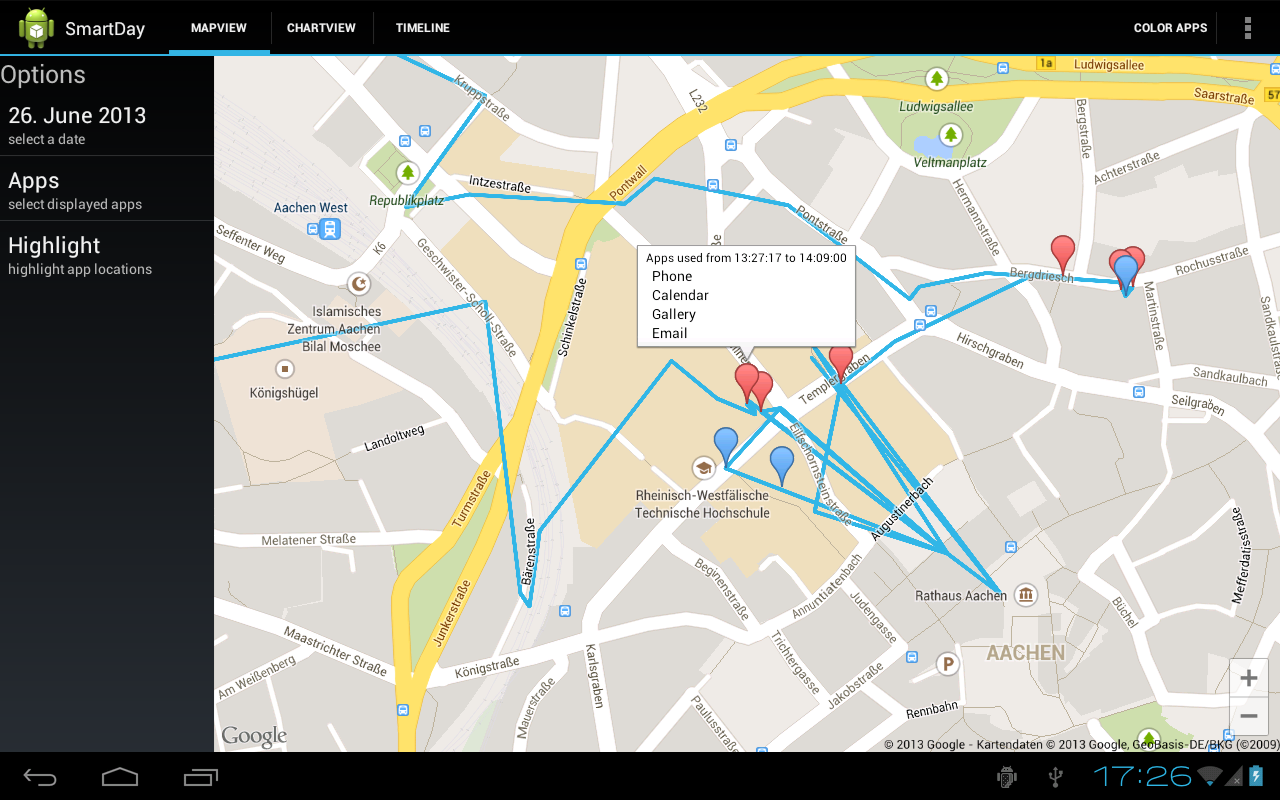
\includegraphics[width=\textwidth]{images/Screenshots/vfinal/Screenshot_2013-08-26-17-20-18.png}
\end{figure}

The \mnote{The options} options on the left side of the view are the date selection option and the application selection option. The first option provides the ability to select a day or a timespan of days which should be displayed in the current fragment. The second option lets the user select applications which are visible respectively not visible in the fragment. Both options were mentioned in the basic layout section as they appear in the sections of the other two views and are not a direct part of the view's  fragment.
The map view also provides an extra option not available in other views. \emph{Highlight} grants the ability to select applications in a dialog fragment, much like the \emph{Apps} option's dialog, which leads to a colorization of markers containing information about the selected applications.

To \mnote{Change appearance with GoogleMap} interact programmatically with the map, one has to obtain an instance of \lstinline$GoogleMap$ by calling \lstinline$getMap()$. With this object one can draw lines, change camera position and add markers. A marker is added at a specific location by calling \lstinline$GoogleMap$'s function \lstinline$addMarker(MarkerOptions)$. It returns an instance of \lstinline$Marker$ which should be stored, as it is needed to modify the marker later and there is no function to obtain set markers from \lstinline$GoogleMap$. The \lstinline$MarkerOptions$ instance contains the adjustments made to a \lstinline$Marker$, like the position or the content of the speech bubble. It is also able to modify the appearance of the speech bubbles which pop up after one taps a marker. In order to create a costume layout, one has to overwrite the function \lstinline$getInfoContents$. To create a line of representing the route of the data, it is possible to use the function \lstinline$addPolyline(PolylineOptions)$. Those polygon lines consists of dots that are connected according to their order of input. Those dots can be defined in the \lstinline$PolylineOptions$ instance that its given as parameter.

Each \mnote{Setting up markers and lines} view fragment in this application implements the \lstinline$OnUpdateListener$ interface. This allows the managing tab listeners, introduced in the basic layout section, to use the same function call for each fragment to provide data and update the view.
When the update function gets called, an array of JSON objects containing data for each day of the timespan is passed. In order to display locations and respectively used applications correct, the JSON objects have to be restructured. Those objects, as mentioned before, are ordered by applications and have to be ordered by location in order to easily access data for the creation of markers which represent places and locations with activities.\\
The algorithm building these new ordered JSON objects constructs them by looping over all applications and their usages and combines application with the same location and stores their name, start and end time. The result is structured as seen in figure \ref{fig:mapsectionjson}.
\begin{figure}
\caption{The Map View JSON Object}
\label{fig:mapsectionjson}
\begin{lstlisting}[language=json,firstnumber=1]
{ "positions":[
    { "highlight": boolean,
      "lat": double,
      "lng": double,
      "start":long,
      "end":long,
      "dates":
        [ double,... ],
      "apps":[
          { "app": string,
            "usage":[
                 {"start": long,
                  "end": long
                 },...
            ]}, ...
      ]}, ...
  ]
}
\end{lstlisting}
\end{figure}

As \mnote{Reordered JSON Object} explained, the events are now ordered by position data. Each position contains information about its latitude and longitude, along with the dates of days at which the location was visited. The fields \emph{start} and \emph{end} represent the earliest and latest time of day, respectively, at which the location was visited. The JSON array \emph{apps} stores the used applications and in case of multiple times it has been used each application in the \emph{apps} array stores its usages. In order to easily determine if an application selected in the highlight option is part of the object, the boolean \emph{highlight} is set to true if one or more applications are contained by it or else it is set to false. In the process of reordering, the algorithm also filters those applications which should hide according to the apps option.

Once \mnote{Creation of marker on polygon lines} the new JSON object representing the data for locations, has been set up, one can start to add markers to the map. First off, the previous added markers and the polygon line have to be removed. To accomplish this part, one has to store the instance of \lstinline$Polyline$ and a list of \lstinline$Marker$ in advance because the Google Maps api does not offer access to the objects through the \lstinline$GoogleMap$ object. For the stored \lstinline$Polyline$ and every element of the \lstinline$Marker$ list, one has to call \lstinline$remove()$ in order to remove the objects from the map. Then, one can loop over the JSON array containing the position data and create \lstinline$MarkerOptions$ instance for every object in the array. Every instance of the \lstinline$MarkerOptions$ is assigned a \lstinline$LatLng$ object storing latitude and longitude, and a title containing a string of the start, end and JSON array \emph{dates} of the respective position in string representation. Each parameter of the string is divided by a pattern in order to be able to split the string. The class \lstinline$MarkerOptions$ also allows to set a snippet which is used to display a subtitle. This snippet stores all used applications,  again divided by a pattern. This has to be done, because the function \lstinline$getInfoContents$ which gets called if the user taps a marker, only provides a \lstinline$Marker$ as input and it only allows to access position, title, id and the snippet. But since one needs to know the dates, times and applications one can either map the marker's id to the respective JSON object and store this, or one can divide the strings in order to recreate the information.\\
After the \lstinline{MarkerOptions} have been created, one calls \lstinline$GoogleMap$'s function \lstinline$addMarker(MarkerOptions)$ and stores the returned marker options in a list.
To create a \lstinline$Polyline$ on has to call the map's function \lstinline$addPolyline(PolylineOptions)$, where the \lstinline$PolylineOptions$ contains a set of \lstinline$LatLng$ objects which get connected in the order in which they were added. The function returns a \lstinline$Polyline$ object which is stored and to can be used to delete it later and is used to change the lines appearance, for example the color and thickness.

If \mnote{Detailed position information} the user taps on a marker, a speech bubble with detailed information about the tapped location pops up. The speech bubble's layout can be changed according to ones needs. In this application, the detailed view is described by an linear layout, showing date and time of visitation on top and all used application names below. The needed information to fill the layout's views are gathered by dividing the strings which are stored in the title and snippet. In addition, the fragment implements the interface \lstinline$OnInfoWindowClickListener$ which provides the function \lstinline$onInfoWindowClick$. This function gets called, once the user taps on the speech bubble and is used to switch the fragments of the application. In this case the user will be presented with the \emph{Timeline} to give him or her a more detailed view of the passed time.

To \mnote{Camera positioning} grant the user a better experience using the map view, one has to take in mind, that the map view's camera position has to be adjusted according to the displayed positions. If one does not take care of the camera, the user would be presented a look at the at the Atlantic Ocean, because the standard camera adjustment looks at zeroth latitude and longitude. To reposition the camera programmatically, \lstinline$GoogleMap$ provides the function \lstinline$moveCamera(CameraUpdate)$. This function sets the camera according to the \lstinline$CameraUpdate$ which in this application is created with a call of \lstinline$CameraUpdateFactory.newLatLngZoom(new LatLng(float, float), float))$. The \lstinline$LatLng$ object defines the position on the map an the float represents the zoom factor, set to twelve if the application readjusts the camera.\\
Repositioning is needed for example if the view visible for the first time or if another view fragment brings up the map view and wants a specific marker in focus.

As mentioned, not \mnote{Receiving data from other views} only can the fragment cause a switch to another view, it can also be switched in by other fragments and be provided with data causing a speech bubble to pop up. The \lstinline$OnUpdateListener$ which provides the function \lstinline$onUpdate$ also provides the function \lstinline$putExtra$. This function is called by the tab listener and granted a JSON object as input. This JSON object should contain informations about latitude, longitude and a time stamp. The function then searches the JSON object containing the applications ordered by location for a position object matching longitude and latitude. If one position is found, all application timespans are searched and if at least one timespan contains the provided time stamp, the index of the position object in the array is used to directly access the respective \lstinline$Marker$ object stored at the same index in the list. This can be done, because first the location ordered array is created and then the marker list is created by sequential working off the array, thus both objects use the same index for their respective location representation. With the marker object then provide the function \lstinline$showInfoWindow$, which leads to the desired pop up of the speech bubble.

Although \mnote{Conclusion} the final version of the map view is not fully as described in the paper prototype section, it still grants an overview of the visited locations. One is able to highlight positions of personal interest and gets detailed information about the applications. It is capable of supporting the displaying of multiple days, which provides the user with an additional ability to adjust the view in such a way, that it fits one's personal needs.



\newpage
\section{Chartview}
Displaying the data in a time opposing manner provides easy opportunity to draw a conclusion about productivity. If one sees at a glance that he or she used a messaging application for 40 percent of the total time, one may wants to rethink his or hers working behavior. An intuitive way of displaying the percentage partition is a pie chart. Pie charts are displayed in the applications view fragment \emph{ChartView}.

The \mnote{AChartEngine library} charts were created with the help of the \emph{AChartEngine} library \cite{achartengine}. The library is open source and offers a variety of different charts and graphs. Working with this library was enjoyable as it has good documentation and large detailed example project which clarified the usage of the library's classes and functions. In order to have access to the library, one has to store the JAR file of it in the \emph{libs} folder of the application's source code and add the library in the project properties. This way the library can be used and is build in to the apk file which installed on the Android device.

The \mnote{Description of the ChartView} ChartView's layout is split vertically into two parts. The left part occupying ca. three fifth of the layout, contains the charts displayed one below the other and are ordered by date in ascending order. Each chart has a title above it displaying the date of the date and the total time of application usage in minutes. The chart itself consists of slices which representing the percentage of of time the respective application was used. Each slice is painted according to the color assigned to the application. Furthermore the slices are labeled with the the percentage and the application name it represents. If one taps on a slice, it gets highlighted by pulling it a bit out of the circle and the view adds new information to the right part of the layout. This part fills the remaining two fifth of the layout and displays detailed information about the currently tapped pie chart slice. These information  are the application name and its usages. Those usages are the start time of the application and the total duration along with text ``show location'' on the time's right. All information are displayed horizontally, ordered by time in ascending order. The described view can be seen in figure \ref{fig:finalchartview}.
\begin{figure}
	\caption{Final version of ChartView}
	\label{fig:finalchartview}
	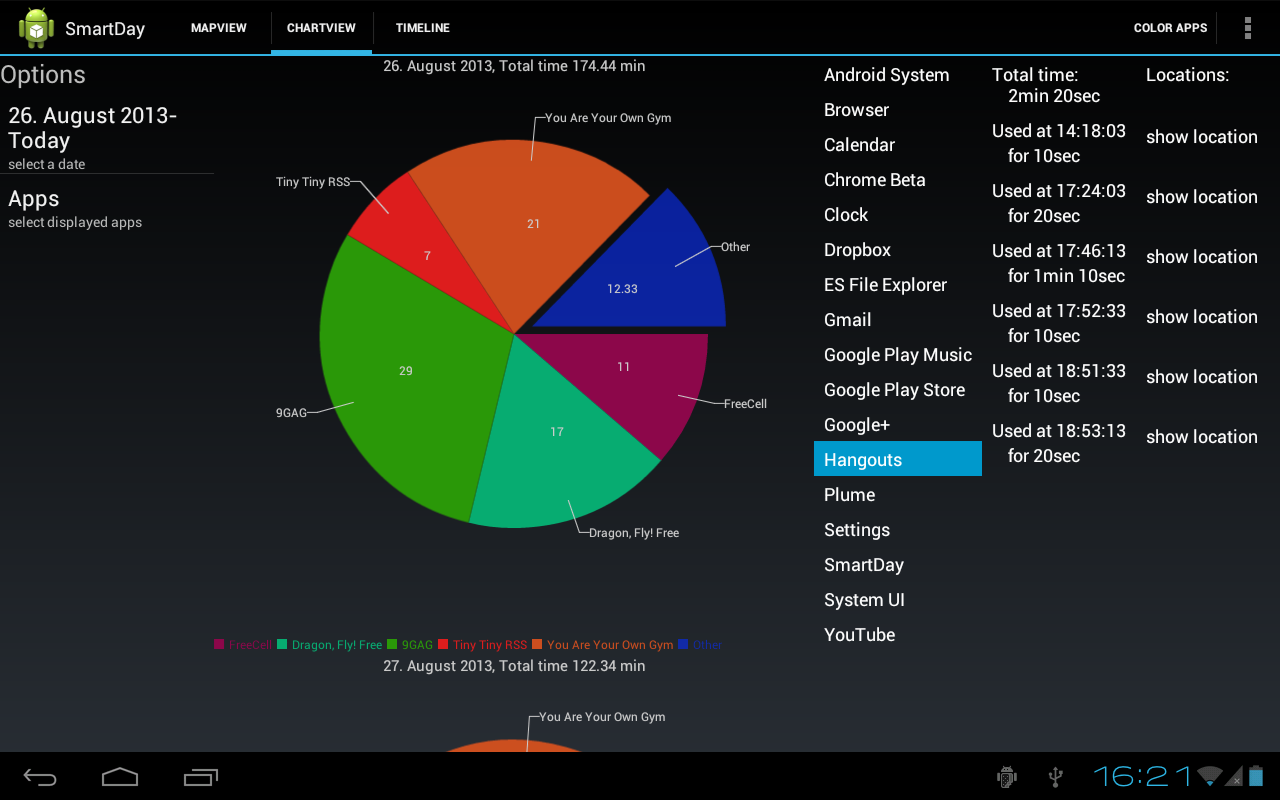
\includegraphics[width=\textwidth]{images/Screenshots/vfinal/Screenshot_2013-08-28-16-21-10.png}
\end{figure}


Options \mnote{Options} affecting the views appearance are the select date option and the select apps option which lets the user choose, what applications to display. Another adjustment that has a effect on the visual appearance of the view is the color apps option. The option was described in section \ref{sec:basiclayout} and allows the user to reassign the colors of applications which are set randomly in first place.

The \mnote{interacting with the view} view offers the possibility to directly interact with it. One can swipe up and down to scroll through the different days represented by charts. Tapping on charts or, in more detail, its slices, will highlight them in the described way. The right side of the layout which provides the detailed information can be used to focus a specific marker in the map section by tapping ``show location'' and it can be used to focus a timespan of the application in the timeline view by tapping on the specific time.\\
In order not to overload the view with too many slices, application with a usage time of lesser than five percent are merged into a slice labeled \emph{other}. Tapping this slice shows all application names represented by the slice on the right side of the layout and tapping on a name reveals their respective time and position information. These information also lead the user to the map view, respectively the timeline.

As \mnote{Differences to the paper prototype} one may have recognized, the view differs from the original concept, in particular, the lacking of position based charts and categorized applications. 
\newpage
\section{Timeline}

